\chapter{相关理论与技术}\label{chap:theories_tech}

\section{Linux调度子系统}

% 内核Core调度流程
% 影响内核调度的关键因素
% - HZ
% - 调度类/机制
% - 调度策略/算法
% - 高质量的操作系统组件,如调度器,则可能需要数十年的时间来完善\citep{agache2020firecracker}

调度子系统是Linux内核的一个重要组成部分,其主要负责在多任务场景下,为系统中的每个进程分配CPU资源。Linux调度子系统通常可分为三层,各层为更上层提供了基本机制,各层的协作为复杂的调度机制的实现提供了可能,如图~\ref{fig:sched_arch}所示,位于最底层的Core调度机制提供了最基本的调度实现,包括抢占调度与非抢占调度,调度类层则针对不同调度目标,提供了包括实时调度、公平调度等特性,并且不同的调度类间存在优先级差异,最上层的调度策略则考虑到不同任务的差异,允许在调度类的基础之上,进一步划分任务的优先级,如在公平调度类中,就区分了NORMAL与BATCH类型的调度策略,同时也提供了系统调用来更灵活地设置任务静态优先级。

\begin{figure}[!htbp]
    \centering
    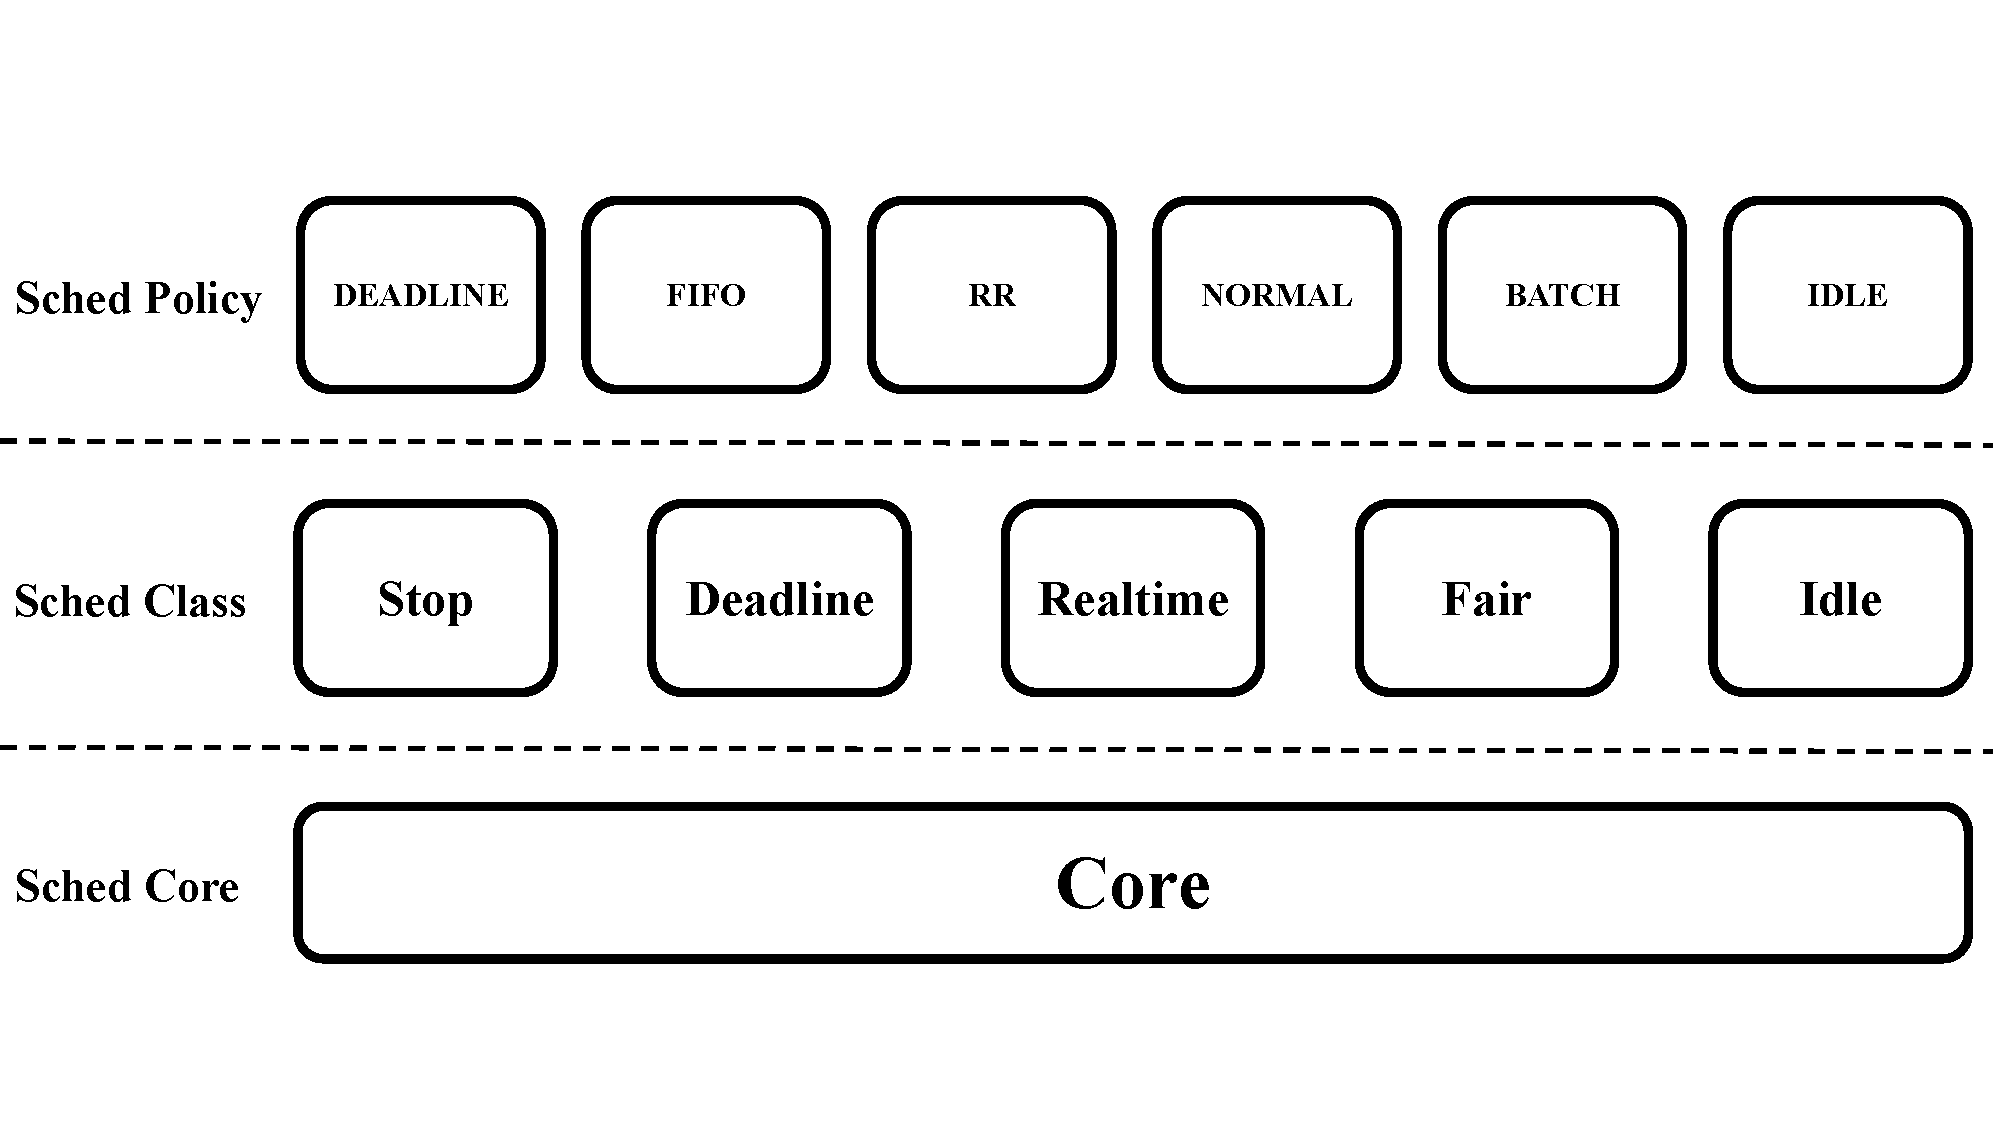
\includegraphics[width=0.7\textwidth]{sched_arch}
    \bicaption{\quad 调度子系统架构}{\quad Scheduling subsystem architecture}
    \label{fig:sched_arch}
\end{figure}

Core提供了最基本的调度框架,是所有调度机制的基本入口。Core调度可分为非抢占式调度与非抢占式两个部分,其中非抢占式调度部分来自于批处理调度,在这一场景中,任务依次执行直到退出。如图~\ref{fig:core_batch_sched}所示,Core调度器需要为新fork出来的任务选择合适的CPU并进行入队,而当任务exit或主动出让CPU之后,则需要重新进行出入队管理,并切换到下一个任务执行,这一过程即是调度循环,如图所示~\ref{fig:shcedule_loop},调度循环通常由中断或系统调用驱动,并在处理完毕到返回用户态之前的时候,通过判断标志位,来决定是否进入到调度循环的主逻辑。抢占调度部分则来自于时间片轮转调度,主要基于时钟中断机制来决策相同队列之上的任务切换,如图~\ref{fig:schedule_tick}所示,在时钟中断处理函数中,会触发Core中的task\_tick的执行,其中就会触发各个抢占式调度类的entity\_tick函数,来对当前任务的记账信息进行更新,当决策判断需要进行抢占时,就会通过Core提供的resched\_curr来设置抢占标记位,从而触发一次调度循环来进行任务抢占。

\begin{figure}[!htbp]
    \centering
    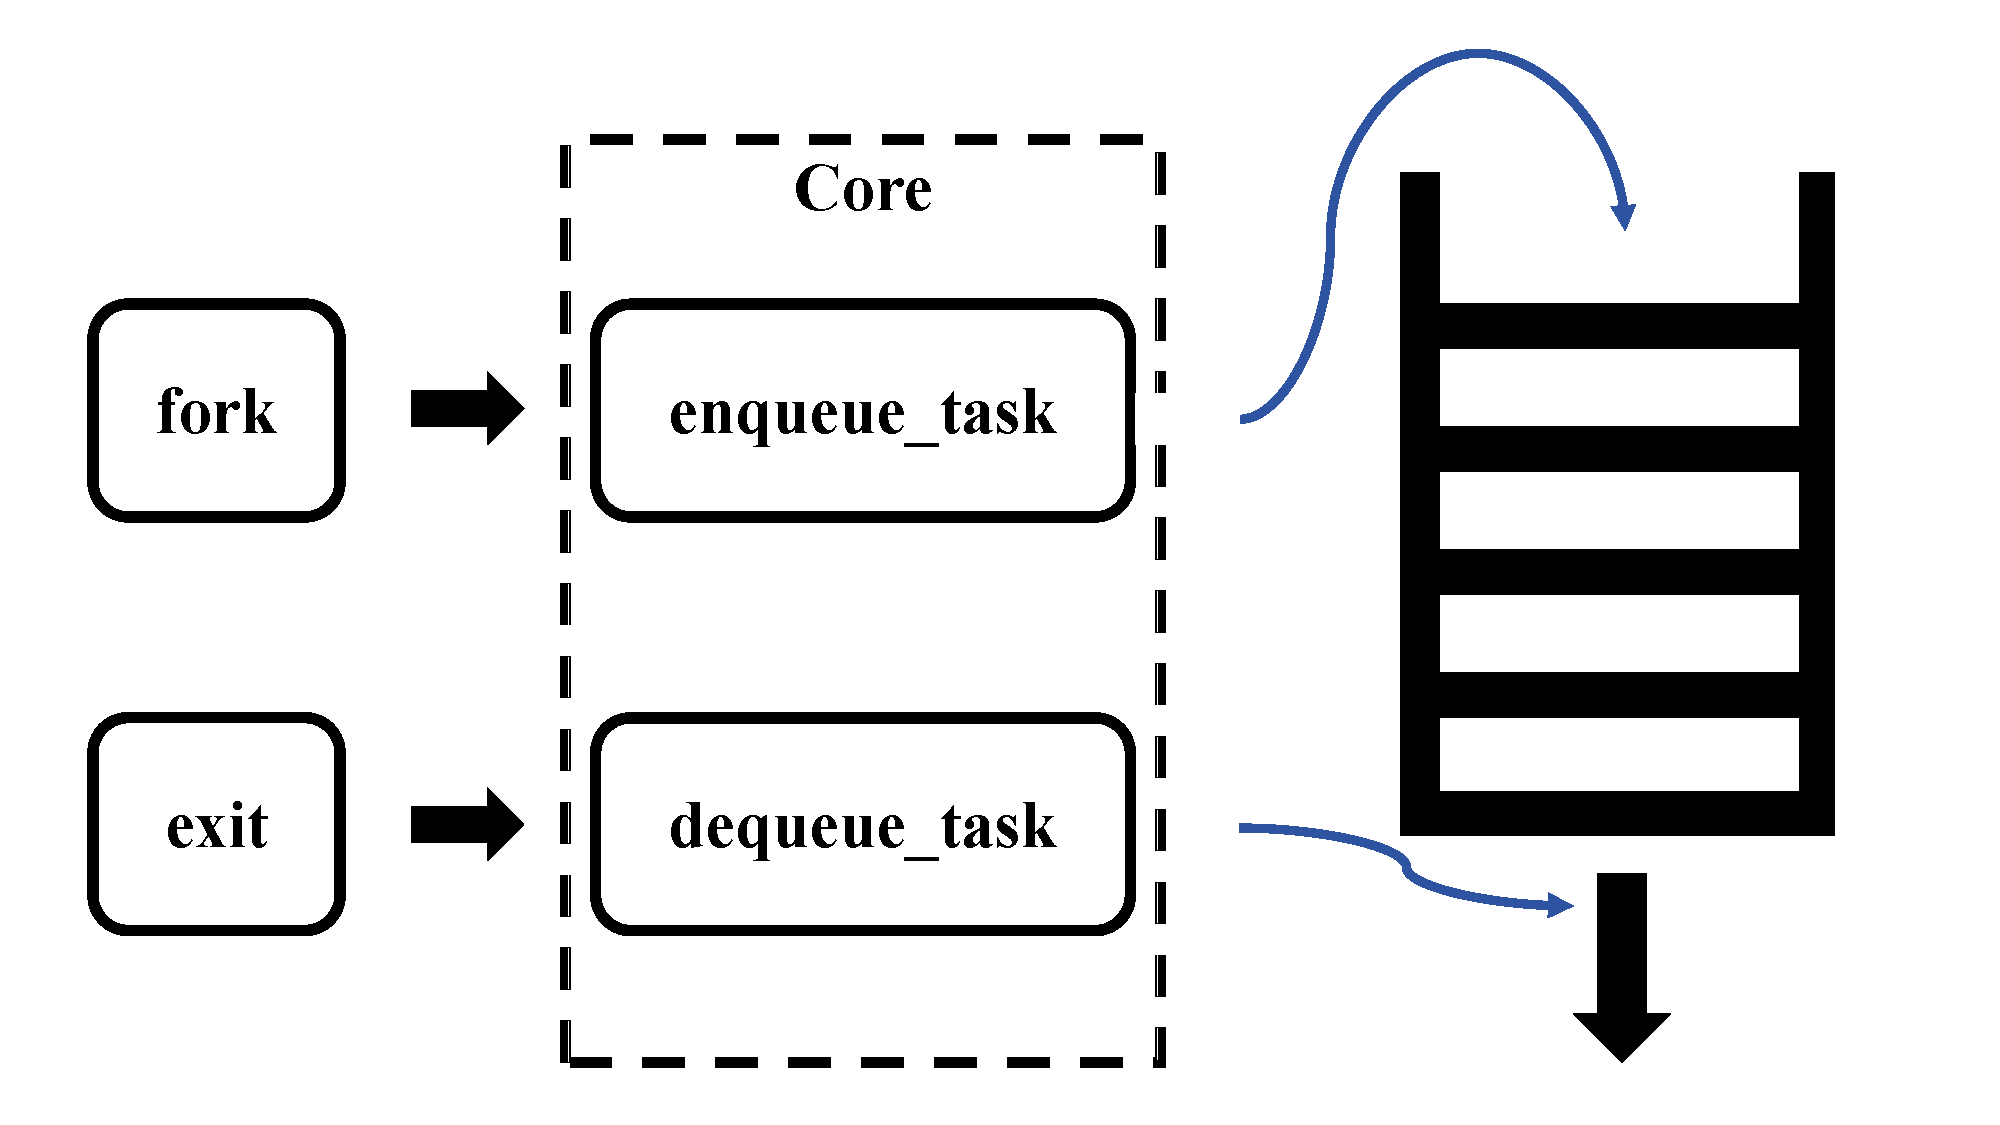
\includegraphics[width=0.8\textwidth]{core_batch_sched}
    \bicaption{\quad Core任务调度}{\quad Core scheduling tasks}
    \label{fig:core_batch_sched}
\end{figure}

调度类层基于Core所提供的基本框架进行设计。当前Linux中主要包含有Stop、Deadline、Realtime、Fair、Idle五大调度类\citep{scheduler},其中Stop调度类的实现最为简单,而其与Core调度的结合便是最早的批处理调度。Fair调度类最为复杂,使用到了大量如红黑树的高级数据结构,并采用了较为复杂的启发式算法与记账逻辑,最终实现了以公平为目标的调度,而其优异的特性使得其一般作为Linux中任务的默认调度类。其余调度类同样以不同的目标进行设计,同时Linux为这些调度类设置了不同的优先级,如图所示~\ref{fig:sched_ext_priorty}, 在每个调度循环中,会从最优先的调度类开始遍历,并依次调度任务执行。

\begin{figure}[!htbp]
    \centering 
    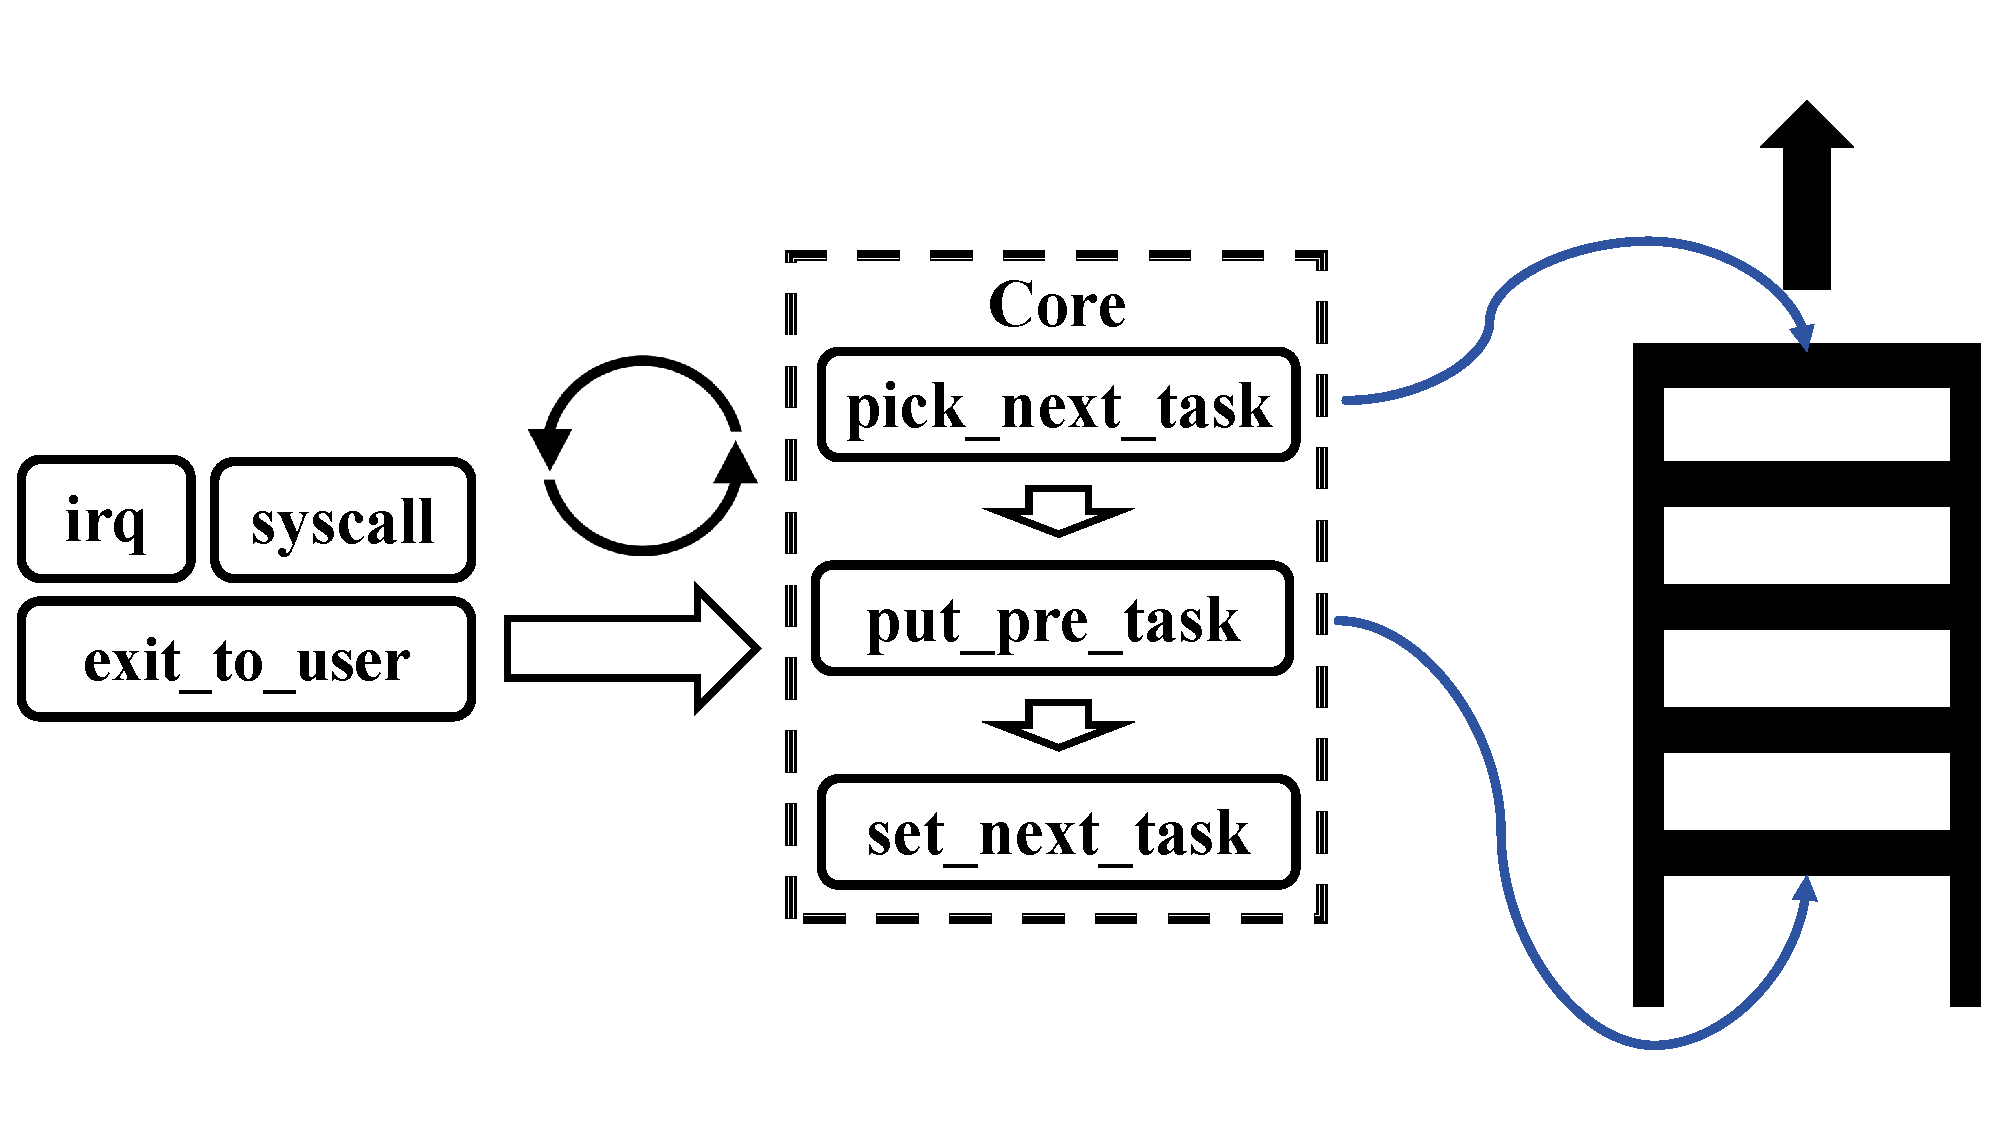
\includegraphics[width=0.7\textwidth]{shcedule_loop}
    \bicaption{\quad 调度循环}{\quad Schedule Loop}
    \label{fig:shcedule_loop}
\end{figure}

调度策略层围绕优先级机制实现,在各个调度类中的实现各不相同。在Realtime调度类中,优先级体现为多个调度队列,选取任务时会从最高优先级的任务队列开始,这保证了高优先级的任务被优先执行,而在同一个任务队列中,调度策略则区分了任务轮换的形式,如FIFO采用先来先执行的逻辑,而RR则通过时间片轮转依次执行任务。而在Fair调度类中,优先级机制的实现则完全不同,这与Fair调度类的算法实现相关,Fair调度类中会为每个任务维护一个vruntime,并在调度时选则vruntime最小的任务执行,优先级体现为vruntime积累的差异,即高优先级的任务积累vruntime的速度会更慢,而基于此Fair调度类提供了NORMAL与BATCH两种调度策略,实质对应为不同的优先级,来提供使用。

\begin{figure}[!htbp]
    \centering
    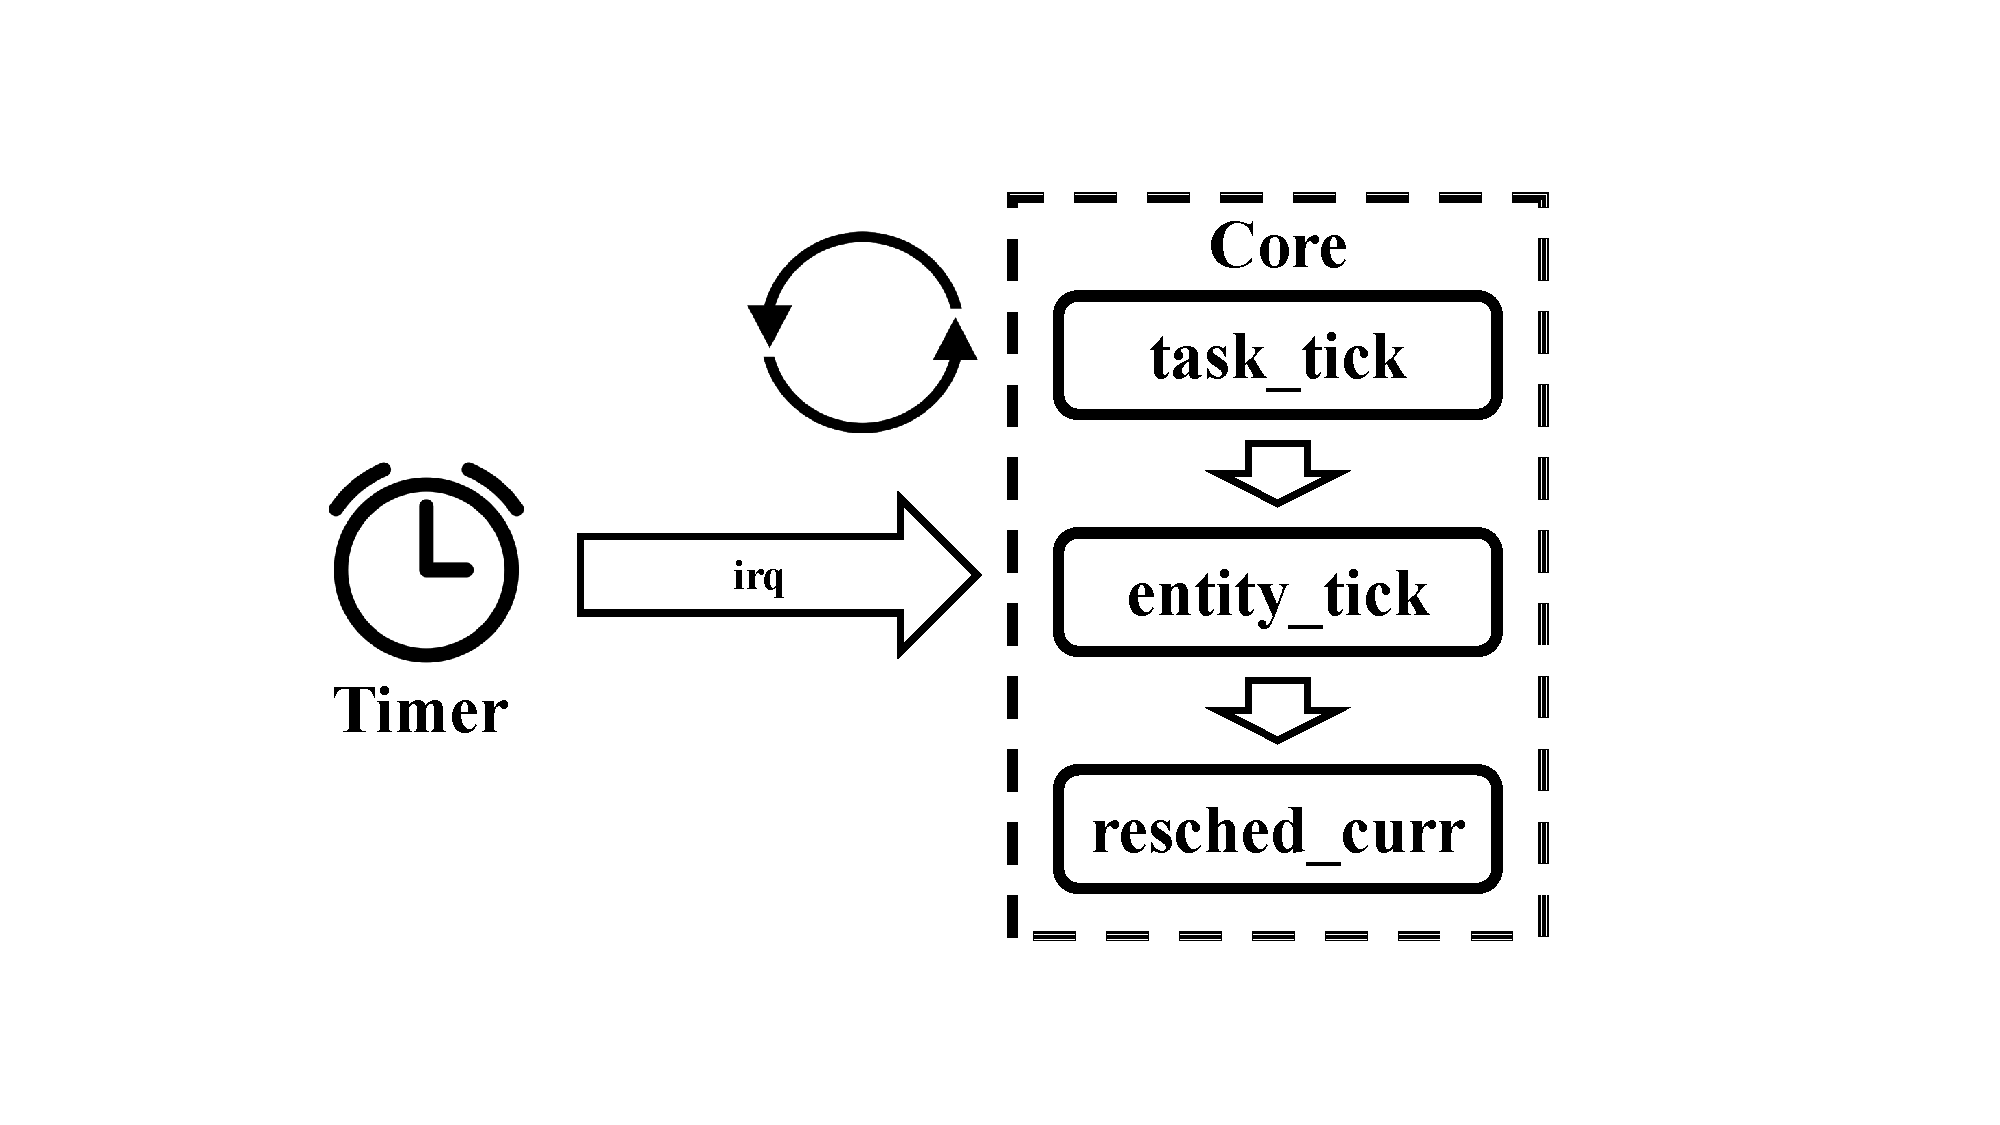
\includegraphics[width=0.9\textwidth]{schedule_tick}
    \bicaption{\quad 抢占调度时钟滴答}{\quad Schedule Tick}
    \label{fig:schedule_tick}
\end{figure}

调度器作为一种质量要求较高的系统组件,通常需要数十年的得带来进行完善\citep{agache2020firecracker},如EEVDF从算法提出到在Linux 6.6中被正式加入就经过29年,并且仍然在不断地被完善。同时调度器作为内核的核心机制,通常牵扯到许多内核中的复杂机制,如各种复杂的同步原语,同时内核环境也为开发者提出了诸多限制,因此在开发、测试与调试上都充满困难\citep{humphries2021ghost}。最后,即便调度器开发完毕,在部署上也存在很高的难度,由于内核无法在运行的状态中对调度器进行修改,因此调度器的部署通常都涉及到任务的迁移,而一旦调度出现错误,则很容易造成较大的损失。

\section{BPF技术}

% 定制内核的需求: 多样的硬件/多样的网络处理模式
% 内核模块: 灵活性高,但不安全,容易引发内核crash风险
% BPF在网络子系统引入,自定义网络包的处理流程
% 逐渐拓展到各个子系统中,但由于内核的审慎地设计,其他子系统中通常用来进行只读操作,如进行监测

eBPF(Extended Berkeley Packet Filter)是Linux内核中的一个轻量级、快速的64位的类RISC虚拟机\citep{sharaf2022extended}。当前eBPF当前已经成为在Linux内核运行时执行不可信的、由用户定义的专用代码的最佳实践与事实标准。其强大的性能、可移植性、灵活性与安全性得到了工业界和学术界的认可,并被广泛地用于更多的领域。

eBPF的前身是BPF(Berkeley Packet Filter),最早由McCanne和Jacobson设计并提出\citep{mccanne1993bsd},起初BPF如其名称所示,用于在Linux网络子系统中对网络包进行灵活处理,而因其本身优异的设计,被Linux内核社区的贡献者扩展到内核的各个子系统中,来对内核功能进行定制化,为了与旧BPF技术进行区分,内核社区将早期的BPF技术成为cBPF(Classic Berkeley Packet Filter),而BPF和eBPF均指代最新的BPF技术,本文在后续说明中也采用这种做法。

BPF本身是一种指令集,最初设计时考虑到安全性与易用性,允许开发者使用C语言的子集进行编写,并能作为一种编译器后端指令集,由GCC等常用编译器编译为字节码\citep{ebpfguidence}。BPF采用字节码的处于两种原因,其一是方便内核验证器对代码进行验证,其二则与Java思想类似,即利用字节码与语言虚拟机的组合提升可移植性。BPF虚拟机运行在内核中,Linux提供了相关的BPF系统调用来将字节码加载到内核中,并附加到代码中声明的钩子函数处,当对应函数触发时,内核态的BPF虚拟机就会执行附加的BPF字节码。整个过程中为了防止加载非法代码,内核首先会在加载BPF程序前对BPF字节码进行验证,判断是否符合在内核中执行的规范,如不允许死循环等,而在内核BPF虚拟机中执行时,会利用JIT技术将字节码映射到本机机器码,从而实现最佳的运行性能。

同作为对内核功能的扩展,BPF技术经常会与内核模块进行比较。相较于内核模块,BPF技术具有更高的安全性,BPF程序安全性体现在三个方面。首先不同于内核模块,BPF程序在编写时所有的对内核数据、地址的访问都需要通过BPF Helper函数来实现,同时,部分BPF Helper函数设计时就考虑到并发性,极大减少了不安全代码的数量。其次,BPF程序在加载时会被内核验证,同时由于运行在虚拟机中,也增强了安全性。最后,BPF程序所能执行的位置由内核提供,这样也大大缩小了危险代码的影响范围。

\begin{figure}[!htbp]
    \centering
    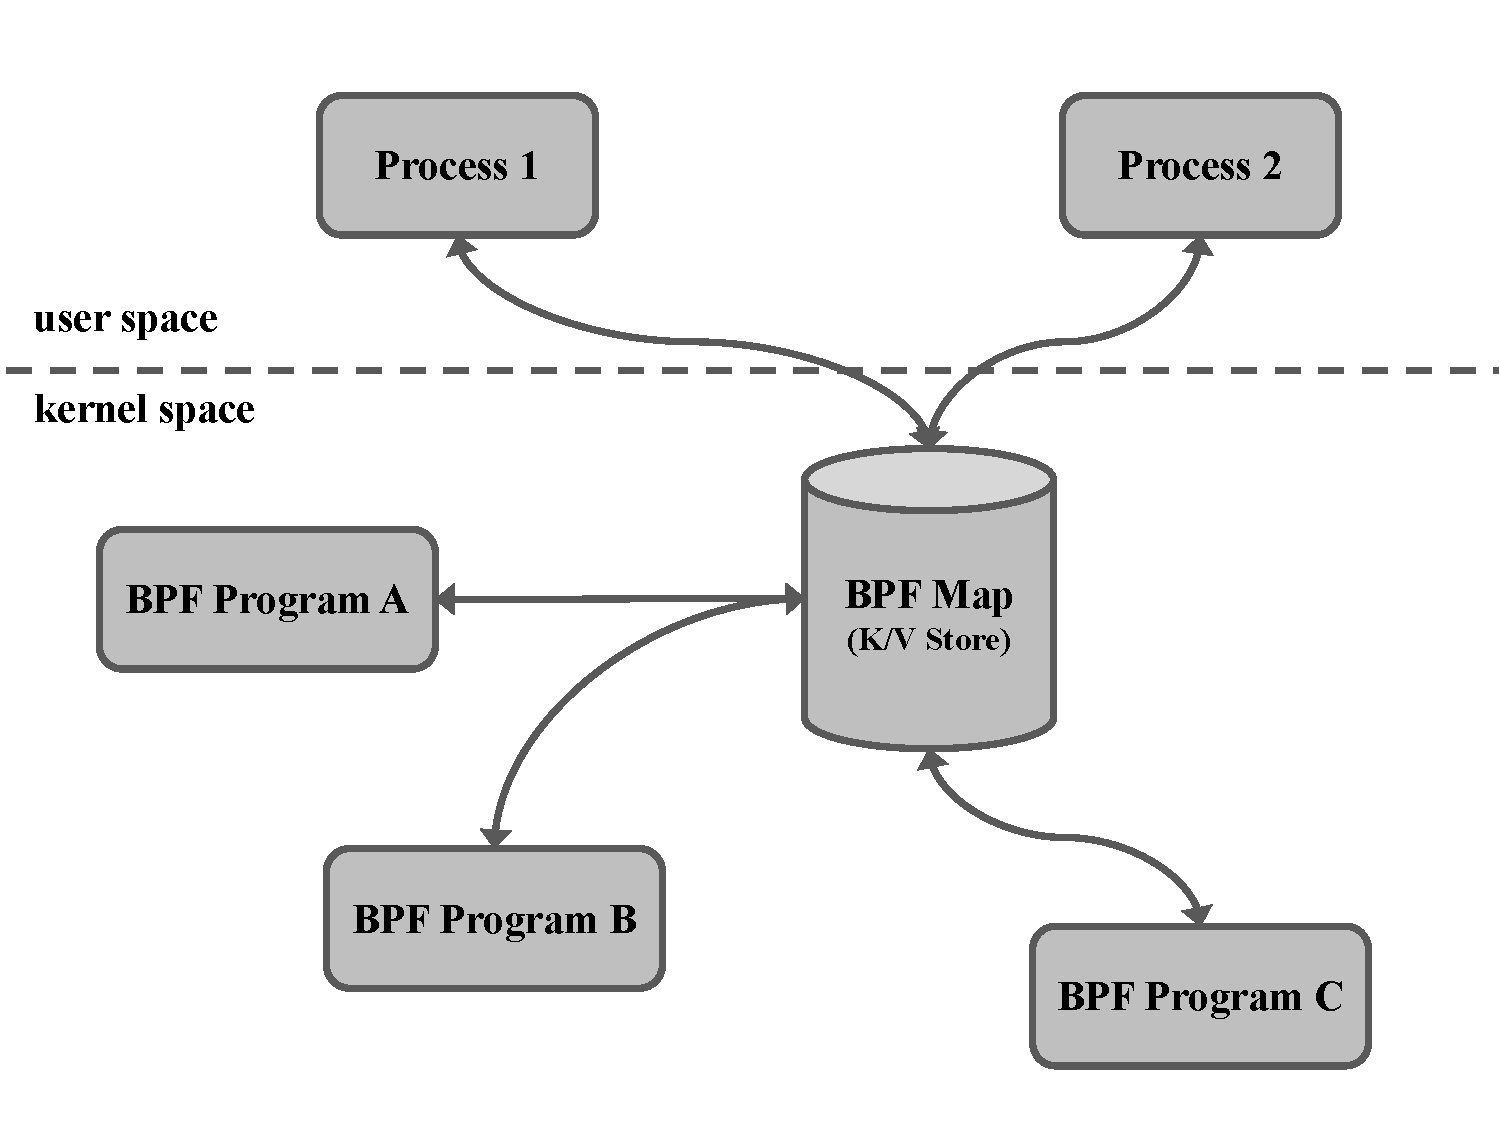
\includegraphics[width=0.6\textwidth]{bpf_user_kernel}
    \bicaption{\quad BPF中用户态与内核态的交互}{\quad Interaction between user mode and kernel mode in BPF}
    \label{fig:bpf_user_kernel}
\end{figure}

同时,BPF技术也具备高度的灵活性。这种灵活性体现在两个方面,首先对于用户态与内核态的交互,BPF技术运行由用户态的程序来加载BPF程序,由于BPF本身是字节码,因此能够借助libbpf等工具来对代码中的部分进行修改,这大大增强了BPF程序的灵活性。其次,如图~\ref{fig:bpf_user_kernel}所示,BPF技术允许通过BPF Map来实现用户态与内核的逻辑交互,一方面,内核态BPF程序所收集到的数据,能够借助BPF Map反馈给用户态程序进行处理,另一方面用户态程序也能通过BPF系统调用操作内BPF Map,对其中的内容进行读写,从而影响内核态BPF程序的行为。其次,BPF技术还允许BPF程序之间的交互,除上述通过BPF Map的交互外,如图~\ref{fig:bpf_to_bpf}所示,BPF程序还能够相互进行调用,从而进行数据传递,或通过多个BPF程序的调用,来突破内核对单个BPF函数的限制,从而实现更加复杂的代码逻辑。

\begin{figure}[!htbp]
    \centering
    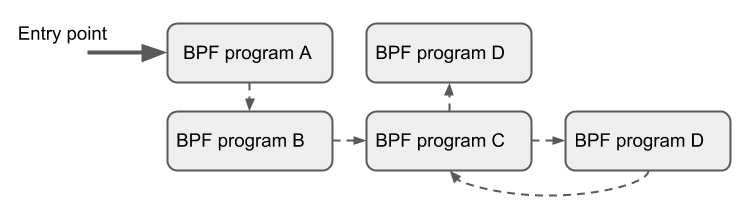
\includegraphics[width=0.7\textwidth]{bpf_to_bpf}
    \bicaption{\quad BPF程序之间的调用}{\quad Interaction between BPF programs}
    \label{fig:bpf_to_bpf}
\end{figure}

BPF字节码通常由内核中的BPF虚拟机解释执行,在一些内核路径上,这种低效的执行方式会严重影响系统性能,而为解决BPF字节码执行的性能问题,内核提供了JIT机制,当字节码首次被加载到内核时,会由内核中的BPF编译器编译为目标体系结构的机器代码,并替换原有的字节码保存在特定内存段中,当对应BPF Hook点触发时,同样先会进入BPF Wrapper函数,并捕获一些栈上数据,但在BPF代码执行处不再唤起虚拟机,而是直接跳转到BPF代码处执行,这使得BPF程序的执行效率大大提高。

然而BPF技术也存在设计上的不足。由于在设计时首要考虑的是安全性,因此BPF程序在编写受到了种种限制,实际上,编写BPF程序所能使用的C语言子集是非图灵完备的,同时BPF程序在栈空间上也有严格的要求。这些限制都极大削弱了BPF程序的表达能力,使得其能够编写的逻辑十分有限。内核社区关注到这一点,并在尝试逐步地减少对BPF程序的限制,并将其引入到更多的子系统中。

\section{可扩展调度类}

Sched Ext是一种可扩展的内核调度器设计\citep{schedext},由Meta以及内核社区的工程师共同设计实现,并已经在Meta的集群中运行与测试。Sched Ext最早提出于2022年,当前尚未合并入内核主线,但Meta与内核社区开发者十分活跃,Sched Ext当前仍然正在积极更新并持续地向内核社区提交Patch。

\begin{figure}[!htbp]
    \centering
    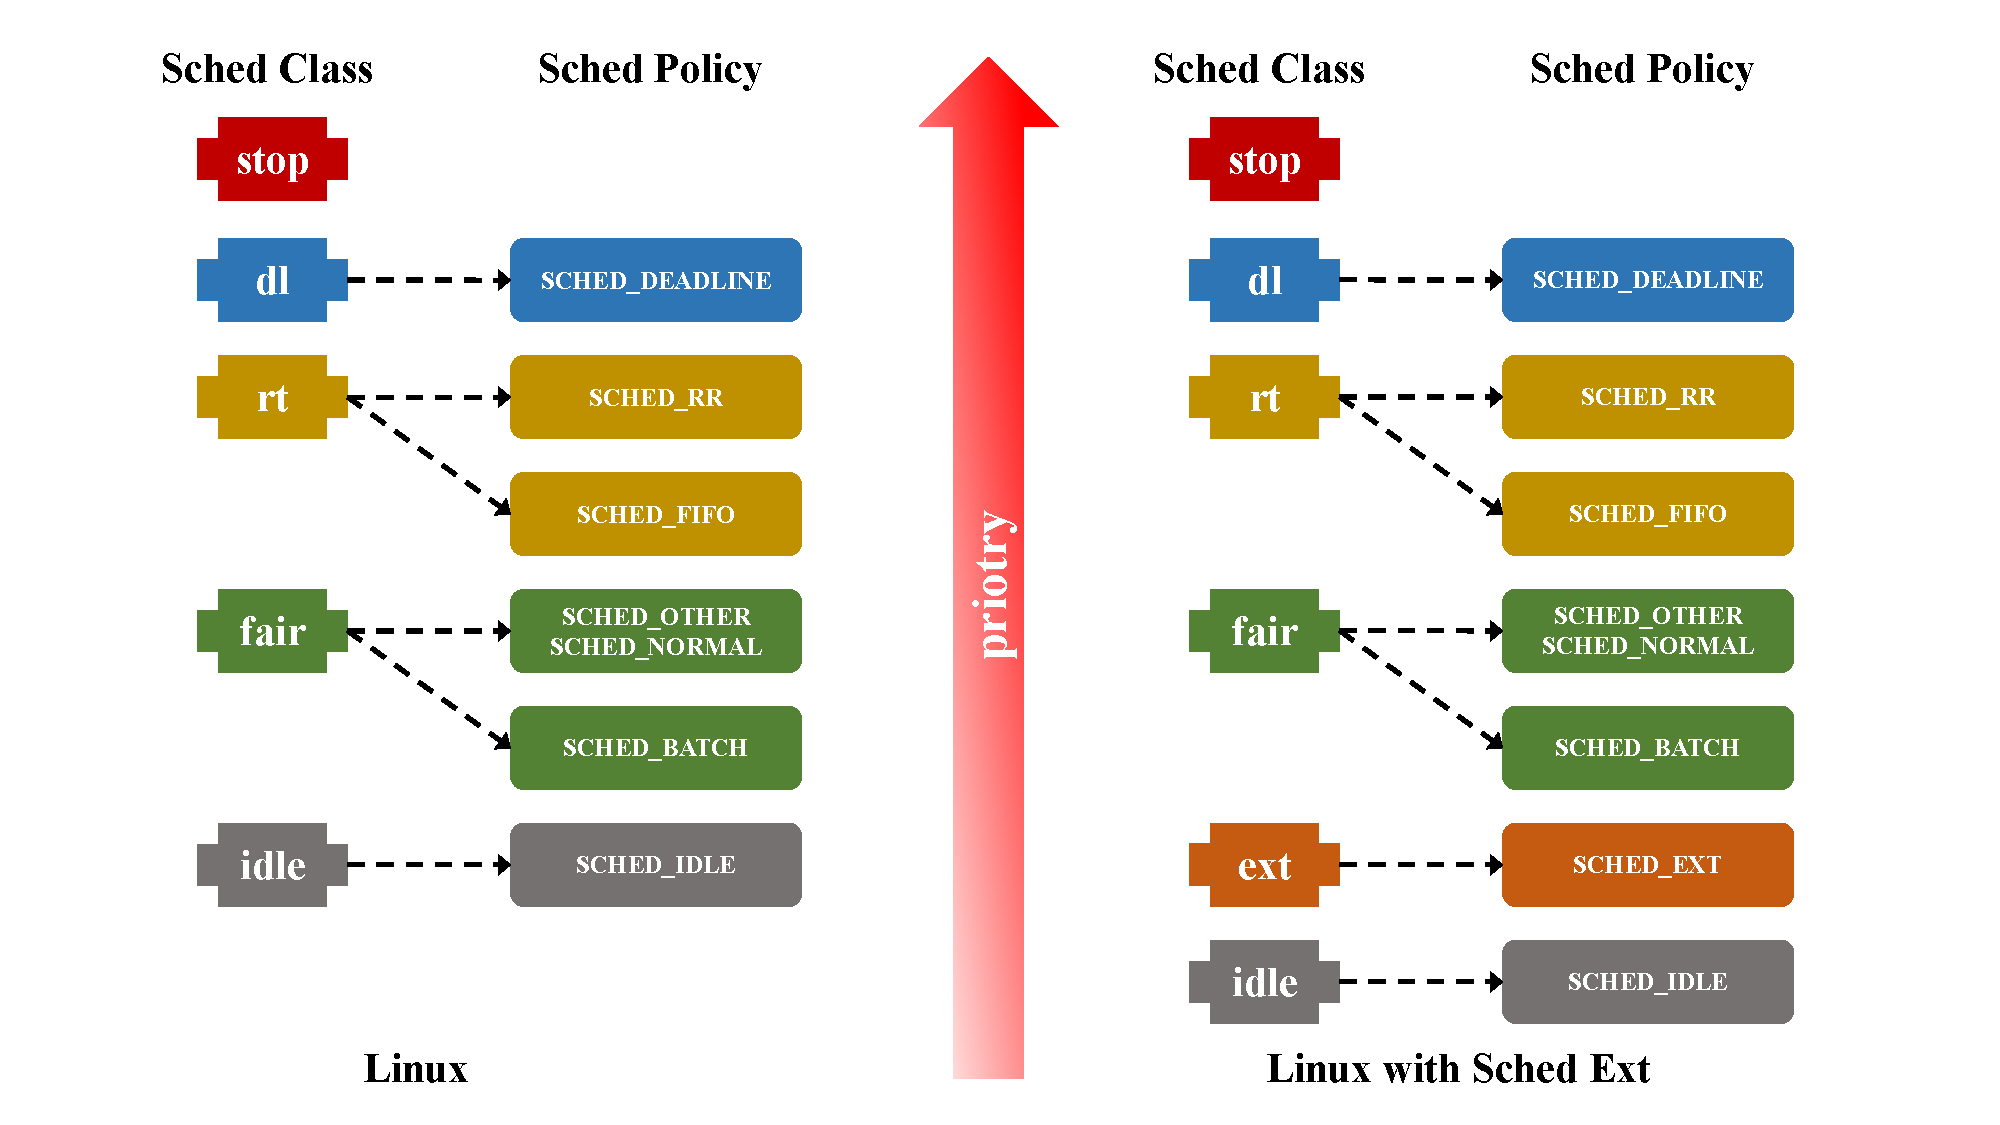
\includegraphics[width=1.0\textwidth]{sched_ext_priorty}
    \bicaption{\quad Sched Ext 调度优先级}{\quad Sched Ext Priorty}
    \label{fig:sched_ext_priorty}
\end{figure}

Sched Ext启发自ghOSt\citep{humphries2021ghost},考虑到内核调度器在开发与部署上的困难与当前数据中心对于定制调度器的需求的不匹配,因此期望设计一种插件化的调度器来提升内核调度器开发的灵活性。相较于ghOSt,Sched Ext在实现灵活调度的机制上存在两点差异,首先,Sched Ext设计之初就尽可能地保持与Linux现有调度机制的兼容性,如图~\ref{fig:sched_ext_priorty}所示的调度类优先级上,Sched EXt的默认优先级在Fair调度类与Idle调度类之间,同时Sched Ext调度类在没有BPF调度器加载时,默认将任务交给Fair调度类处理,通过以上两种处理,使得在使能Sched Ext时几乎不会对现有的调度机制产生影响。其次,Sched Ext调度的实现不局限于用户态,Sched Ext选择BPF来作为调度类的可扩展机制,通过增加BPF的特性,如增加Helper函数,扩展Map类型等,来使得其能满足编写调度器的基本要求,这样的设计使得一方面,开发者可以利用BPF的表达能力在内核态定制调度机制,另一方面也可以利用BPF程序与用户程序的互通性,在用户态设计调度器从而避开内核态编程的限制。

Sched Ext与其他调度类一致,实现了调度类所需要的全部方法。但与其他调度类不同的是,Sched Ext的调度过程需要与BPF Scheduler进行协作完成。而为让BPF Scheduler介入调度过程,Sched Ext调度类中首先定义了调度队列DSQ,通常每个CPU上都会有自己的Local DSQ,BPF Scheduler则可以拥有数个DSQ,任务在不同的DSQ之间流转,而只有在CPU Local DSQ上时,才有被执行的机会,同时,Sched Ext围绕DSQ管理以及BPF与CPU的互动定义了一些列BPF Helper函数,如图~\ref{fig:sched_ext_helpers}所示,这些Helper函数支持BPF Scheduler完成整个调度过程:

1)scx\_bpf\_create\_dsq: 定义一个DSQ(调度队列)来对任务进行管理。DSQ是BPF Scheduler管理任务的核心, BPF程序中可以保有不止一个DSQ,DSQ之间通过ID来进行区分,同时通过NUMA亲和性能够来保证访问DSQ内存的效率。

2)scx\_bpf\_dispatch、scx\_bpf\_dispatch\_vtime:将任务调度到DSQ中。调度逻辑中可通过ID来指定目标DSQ以及任务的运行slice,其中slice可以设置为无限,此时任务不会被同队列中的其他任务抢占,而由BPF程序来决策抢占的时机。调度的任务通常以FIFO的形式入队,Sched Ext也提供了基于vtime的类CFS队列,以满足不同的BPF调度器的设计需求。

4)scx\_bpf\_dispatch\_nr\_slots:查看CPU可调度的任务槽数。允许BPF程序检查当前CPU上可承载的任务余量,避免BPF Scheduler向目标CPU调度过多的任务。

5)scx\_bpf\_dispatch\_cancel:撤销最近向CPU调度的一个任务。当任务的CPU亲和性发生变化时,BPF Scheduler原先调度的任务就应当进行变化,而此Helper函数便于BPF Scheduler撤销先前的调度决策。

6)scx\_bpf\_consume:将BPF scheduler管理的任务调度给CPU。Sched Ext中的任务需要经过从BPF Scheduler的调度队列到CPU本地调度对队列的过程,这一过程的通过此Helper函数完成。

7)scx\_bpf\_kick\_cpu:激活CPU的重调度。BPF程序能够通过此Helper函数唤醒一个idle CPU或者让繁忙的CPU进入调度循环中,其中为避免唤醒的时间过程,采用向中断队列添加延时任务的形式异步地设置唤醒任务,而在唤醒的过程主要通过Core中提供的resched\_curr完成。

8)scx\_bpf\_pick\_idle\_cpu:找到一个空闲的CPU。根据不同的调度目标,调度器应当避免任务过度的集中于同一个CPU,BPF Scheduler可以通过此Helper函数找到一个空闲CPU,将任务调度到此CPU上,并结合其他Helper函数来唤醒CPU。

\begin{figure}[!htbp]
    \centering
    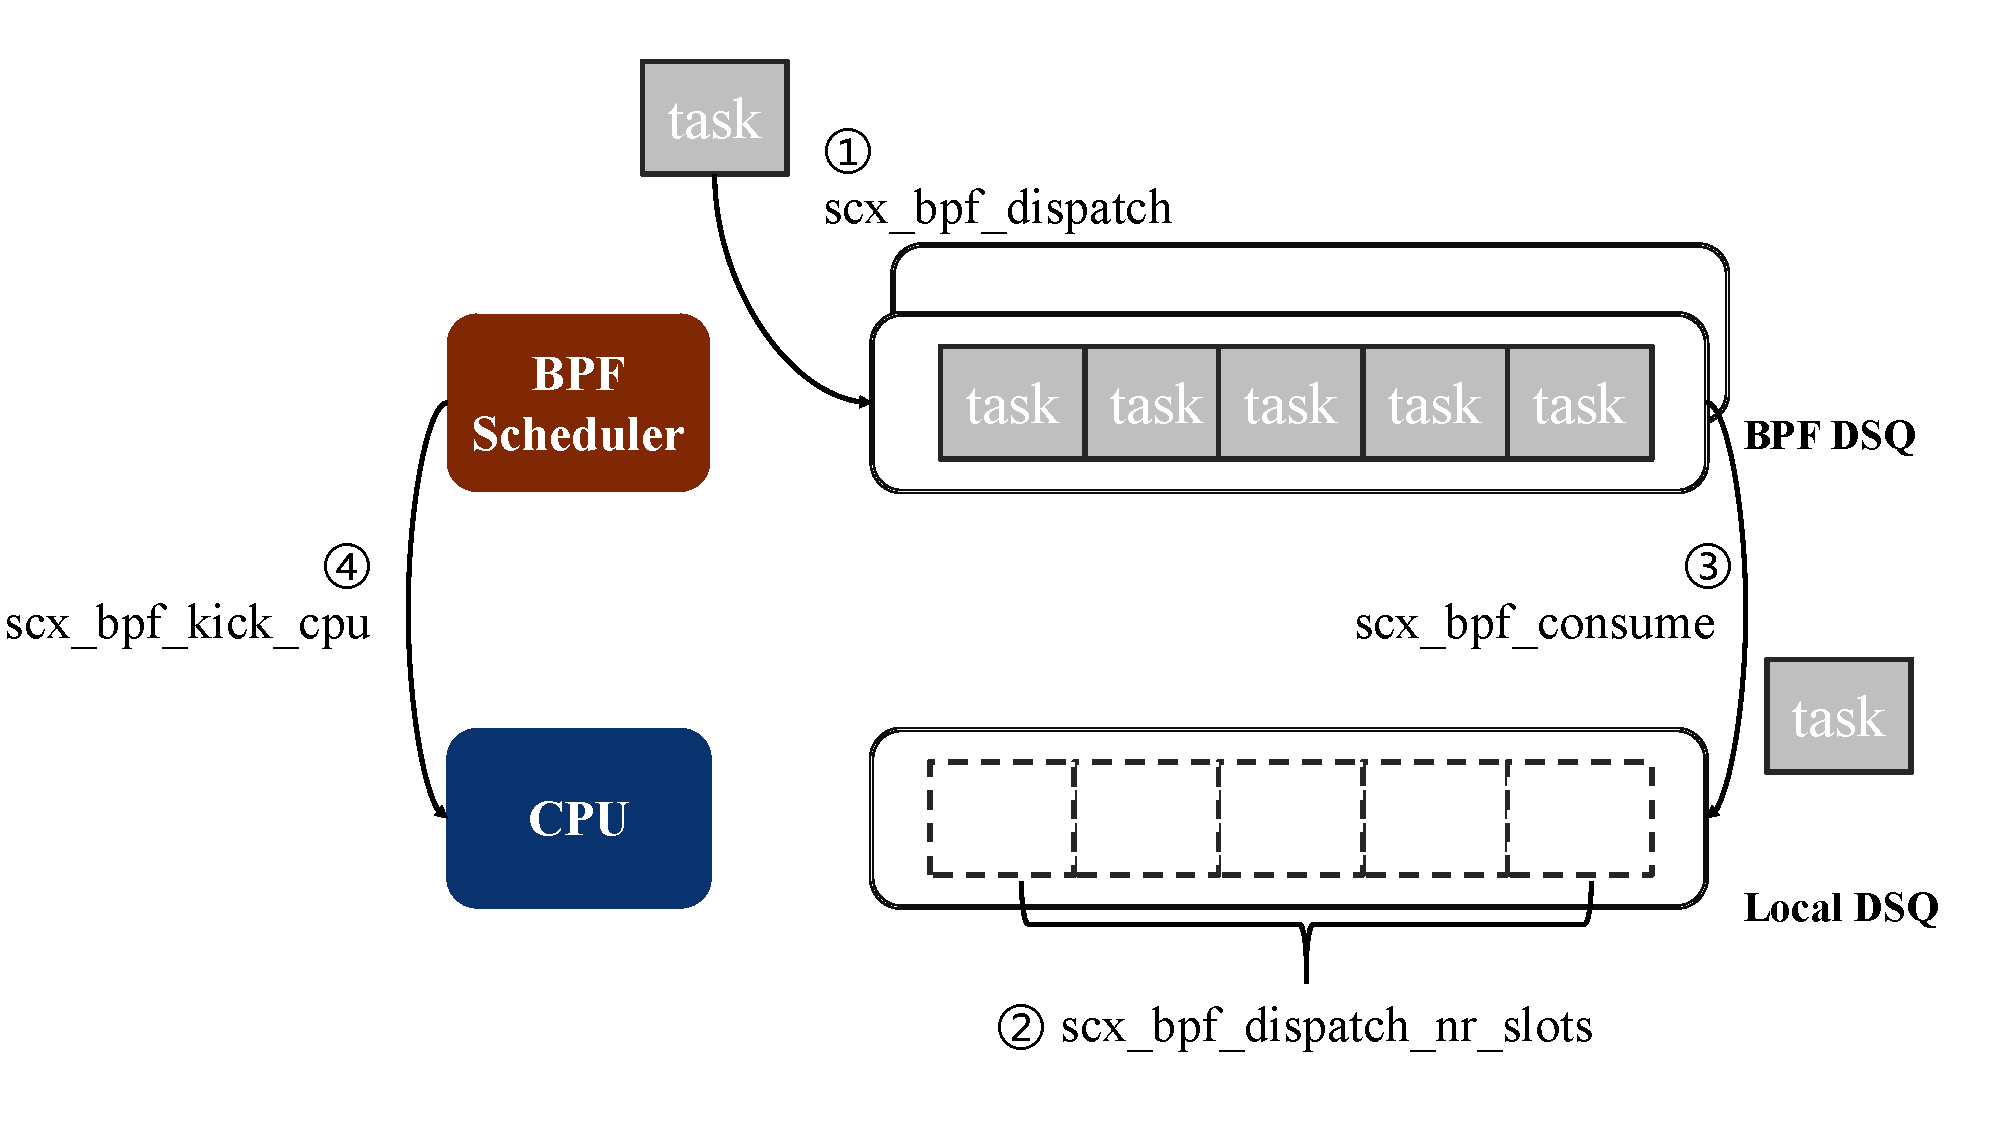
\includegraphics[width=1.0\textwidth]{sched_ext_helpers}
    \bicaption{\quad Sched Ext BPF Helper 函数}{\quad Sched Ext BPF Helpers}
    \label{fig:sched_ext_helpers}
\end{figure}

Sched Ext调度类的调度过程与Linux Core调度框架类似,如图~\ref{fig:sched_ext_arch}所示,Sched Ext调度类本身实现了基本的调度类函数,用以承担基础的调度任务,同时作为调度的入口,允许BPF Scheduler在调度的各个关键路径上辅助进行决策。而为实现以上设计,Sched Ext中定义了sched\_ext\_ops抽象,每个BPF Schedueler都需实现其中的全部或部分函数,从而能够在调度的过程中发挥用。

1)select\_cpu:为唤醒的任务选择一个CPU。这一过程通常发送在SMP系统中,需要考虑任务的特性以及CPU的负载情况,选择的结果会影响到系统总体的性能,因此BPF所实现的逻辑不一定是最终的调度结果,实际的调度决策还会结合调度类本身的决策与BPF的决策。

2)enqueue:处理任务的入队。调度类所管理的任务就绪时,会在入队的关键路径上触发BPF enqueue的执行,BPF中可将任务通过Helper函数发送到DSQ中,并进行后续的管理。

3)dequeue:处理任务的出队。当需要对任务的调度属性,如优先级,进行修改时,便会触发任务出队逻辑,此时BPF中可以自定义优先级的更改逻辑,从而实现自定义的优先级功能。

4)dispatch:处理任务的调度。BPF可以通过创建DSQ来持有任务,同时每个CPU也拥有自己的Local DSQ来保存要执行的任务,当CPU的Local DSQ为空时,就会触发BPF的任务调度,期望从BPF的DSQ中获取将要执行的任务。BPF可以一次性调度多个任务,从而增加调度的效率,而任务的选择则完全由BPF程序决定。

5)runnable、running、stopping、quiescent:追踪任务的状态。任务通常会在如下三种情况进入Runnable状态,首先是被唤醒时,如从等待IO的状态中恢复,其次是从其他CPU迁入时,以及从队列中暂移后恢复时,如修改任务优先级时,这些情况通过flag进行区分,并触发runnable的执行,quiescent的触发与上述时机完全相反,其他函数则在更细致的时机触发以反映任务的状态,其中running对应任务将要在CPU上运行时,stopping对应任务将要停止运行时。BPF通过这些函数来追踪任务的状态变化,从而辅助进行自定义的调度过程。

6)yield:让出CPU资源。Linux提供了sched\_yield系统调用,允许任务主动放弃CPU资源,通常用于多线程中。sched\_yield并不保证线程组中的其他线程立即执行,而是将决策交给调度器,Sched Ext中此决策过程可完全由BPF程序实现。

7)init\_task、exit\_task: 追踪任务的创建与退出。调度类中每当有任务新创建或退出时触发,BPF可追踪这些事件,从而能够在BPF Scheduler中为每个任务定义额外的信息用于后续的调度过程。

\begin{figure}[!htbp]
    \centering
    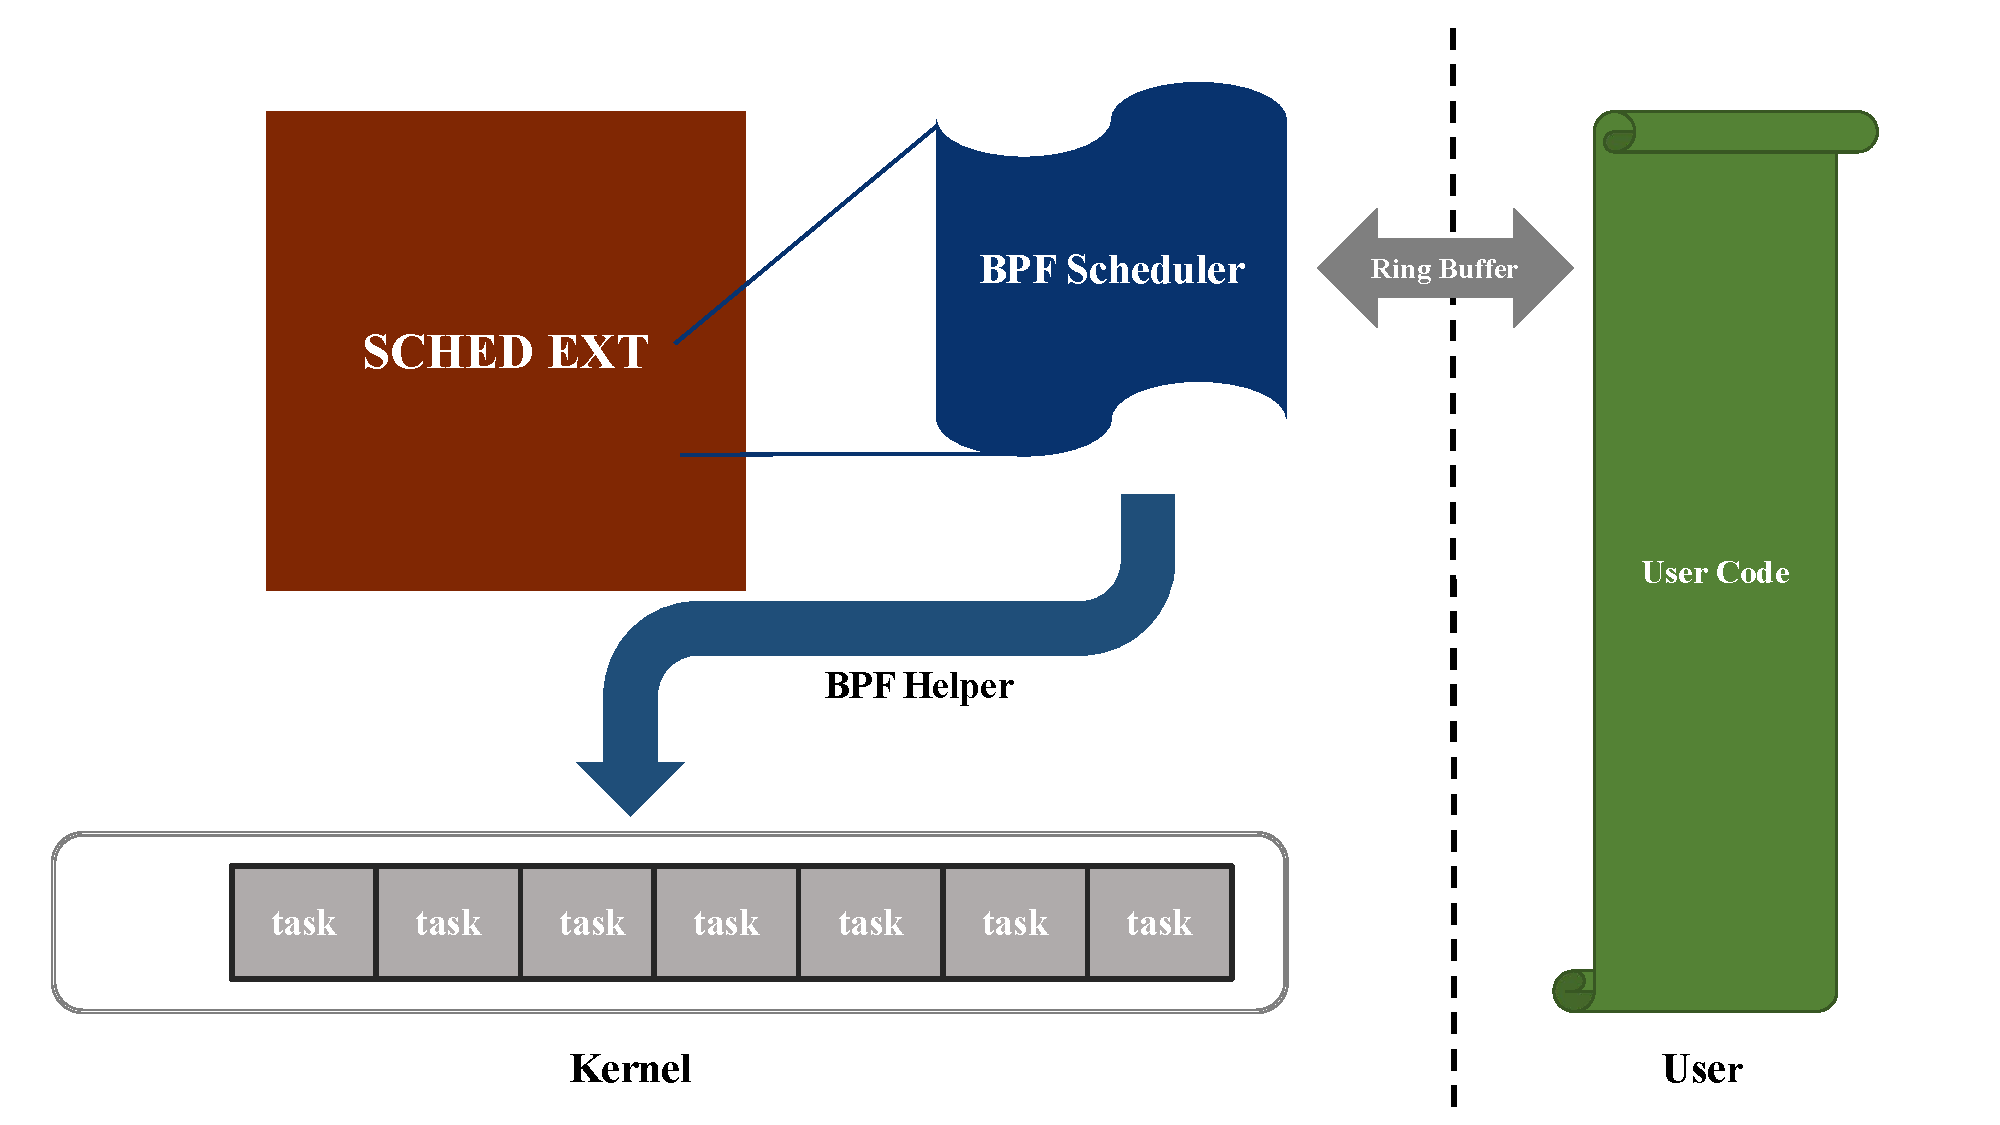
\includegraphics[width=0.7\textwidth]{sched_ext_arch}
    \bicaption{\quad Sched Ext架构}{\quad Sched Ext Arch}
    \label{fig:sched_ext_arch}
\end{figure}

BPF Schedueler的引入为开发者提供了丰富的手段来定制Sched Ext调度类的调度行为。首先最直接也是最为简单的就是仅设置Ext调度策略,即不加载任何BPF Scheduler类,此时即便任务的调度策略是Ext,但由于并未加载有效的BPF Scheduler,Sched Ext会将任务的调度类会默认设置为Fair调度类,并在Fair调度类的调度队列中进行调度,而Sched Ext仅会维持一些追踪任务的必要信息,从而保证了任务的执行。其次,开发者可以编写BPF Scheduler,并经由系统调用将BPF程序加载到内核,BPF Scheduler通常需要JIT来保证运行性能,Sched Ext调度类在初始化开发者定义的BPF Scheduler时,会对所有Ext调度策略的任务进行初始化,并交由BPF Scheduler进行管理,同时,为了管理方便,开发者也可以设置初始化参数,以接管所有Fair调度类的任务。最后,即便JIT之后的BPF程序运行在内核态运行效率非常高,但受限与内核编程环境,无法实现较为复杂的逻辑,然而BPF程序的优势在于能够与用户态程序进行交互,Sched Ext也为此设计了一套用户态调度器的开发框架,用户态程序通过监听BPF MAP来获取BPF Scheduler中的调度信息,并在用户态进行决策,将结果写回BPF Map,而BPF Scheduler在合适的时机将调度结果进行实施,通过这种用户态与内核态BPF Scheduler协作的方式,使得大部分的调度逻辑能够在用户态完成,从而支持更灵活的调度策略。

\section{沙箱技术}

% 系统级沙箱(虚拟机),容器级沙箱(进程)
% 安全性: 虚拟机 > 沙箱
% - 容器类沙箱缺乏调度机制的支持,而对调度机制的修改需要更安全的沙箱环境来限制风险的传播

沙箱技术是一种安全机制,用于隔离运行环境,以便在受限的环境中执行不受信任的程序或代码,并防止这些程序或代码对主机上其他任务造成影响或危害。沙箱是通过在受限的操作系统环境中执行软件来实现的,并对软件所能使用的资源,如CPU、内存、网络等进行限制。沙箱技术为在数据中心中安全地运行各种各样的应用提供了基础,而在数据中心中,常见的沙箱技术包括虚拟机技术与容器技术。

虚拟机技术是数据中心应用最广泛的沙箱技术,通常指通过软硬件的手段,在已运行的系统中模拟出一个硬件环境,并能够支持运行其他系统。虚拟机技术最早提出于\citep{bugnion1997disco}, 用于解决操作系统迭代速度与硬件更新速度不匹配的问题,并希望依托虚拟设备与虚拟机环境,来提升操作系统的迭代速度。而随着虚拟化技术的不断发展,虚拟化开销也逐渐降低,其中软件上,从运行在裸金属上的Type 1虚拟化技术Xen\citep{barham2003xen},到能够将Linux转化为一个Hyeprvisor的Type 2虚拟化技术KVM\citep{kivity2007kvm},虚拟化软件技术的不断发展使得虚拟机的管理越来越简单,而在硬件上,基于SRIOV的设备直通手段\citep{dong2012high},让虚拟机能够直接接触物理设备,从而达到几乎与裸金属操作系统相近的性能。同时虚拟机具备较高的隔离性,能够较好的处理多租户场景下的安全性问题,以上这些为虚拟机在云厂商中较长时间的广泛使用提供了基础。

容器技术期望提供一种进程级别的沙箱,来隔离运行在同一系统上的不同进程。程序的执行依赖一定的运行环境,Linux早期的发展过程中,由于包管理工具的不成熟,使得不同程序之间会相互污染运行环境,造成程序的运行错误或失败,为解决此问题,Linux提供了chroot工具以及相关的系统调用,允许为程序设置不同的根目录,从而让不同的程序运行在满足各自运行环境的根目录中,解决相互之间的依赖污染问题。chroot实质是一种文件系统的隔离机制,而后在Linux的不断发展过程中,越来越多的隔离机制被实现,其中Cgroup与Namespace机制构成了现代容器技术的基础。Namespace技术提供了Mount、UTS、IPC、PID、Network及User等系统资源的隔离,使得容器中的进程几乎认为自己运行在一个独立的系统环境中,而Cgroup技术则提供了CPU、Memory、BlkIO、NetIO、Devices等硬件资源的隔离,使得容器中的进程能够运行在一个受限制的硬件资源环境中。Overlayfs技术能够将多个目录文件叠加为一个统一的目录文件,并允许各层之间有不同的读写行为,同时借助COW(写时复制)来解决各层文件共享的问题,而这一技术为容器镜像技术提供了基础,而借助标准化的OCI镜像,容器得以方便地在不同的发行版、软件环境的Linux系统中传播。容器的易用性催生了容器编排技术,而以Kubernets为主的容器编排技术在数据中心中占有越来越多的比例。

容器在本质上仍然是进程,因而在执行效率上高于虚拟机,但由于进程共享了相同的内核,因而不可避免地保有进程的安全问题,而这点在多租户场景的云环境中尤为凸显。现代容器技术提供了各种各样的手段提升容器的安全性,如限制容器中进程能够使用的系统调用等,然而这种方式牺牲了容器的通用性,容易导致部分容器的运行异常。安全容器的提出就试图解决这一问题,安全容器本质上是一个高度裁剪的虚拟机,运行着一个同样高度裁剪的内核,这样的处理大大精简了虚拟化环境,从而能够在提升虚拟机启动速度的同时,减少虚拟机本身的内存占用,同时,绝大多数的容器镜像都包含了一个较为完整的根文件系统,稍作处理后就可以作为一个虚拟机镜像来提供虚拟机使用。安全容器作为一种沙箱技术,结合了虚拟机的强隔离性与容器的易用性,在虚拟机运行时上,阿里的RunD\citep{li2022rund}、AWS的Firecraker\citep{agache2020firecracker}等轻量级虚拟机运行时大大降低了虚拟化的额外开销,而基于轻量级虚拟机技术所构建的安全容器如gVisor、KataContainer\citep{randazzo2019kata}等也逐渐在数据中心中应用。

\section{本章小结}

本章节首先介绍了Linux中的调度子系统以及eBPF技术,说明了当前Linux调度子系统的基本原理以及发展状况,并阐述了eBPF技术作为一种集性能、灵活性于安全性于一体的内核扩展机制的工作原理,随后介绍了将eBPF技术引入到调度子系统的可扩展调度类Sched Ext,分析了其核心的BPF Scheduler原理,其所带来的灵活的内核调度机制设计,有利于加速当前Linux调度子系统的迭代,并为在各种场景下的定制化调度优化提供了可能。最后介绍了常见的沙箱技术,以容器技术、虚拟机技术、安全容器技术为主,分析了不同沙箱技术所重点解决的问题,以及存在的优劣势。以上这些相关技术构成了后续Control Zone设计实现的基础。